\subsection{向量丛的态射}

7.2.1. 设 B 和 B' 是两个流形，f 是从 B 到 B' 的态射。设 M 是以 B 为基底的向量丛，M' 是以 B' 为基底的向量丛。如果满足以下条件，则称从 M 到 M' 的映射 g 为向量丛的 f-态射：

对于每个点 \(b_0 \in \mathbf{B}\)，存在一个向量丛图 \(t = (\mathrm{U}, \varphi, \mathrm{F})\)，它属于 \(\mathbf{M}\)，在点 \(b_0\) 处；存在一个向量丛图 \(t' = (\mathrm{U}', \varphi', \mathrm{F}')\)，它属于 \(\mathbf{M}'\)，在点 \(f(b_0)\) 处；以及一个映射 \(\lambda\)，其类为 \(\mathbf{C}'\)，从 \(\mathbf{U}\) 到 \(\mathcal{L}(\mathbf{F}; \mathbf{F}')\)，使得 \(f(\mathbf{U}) \subset \mathbf{U}'\)，并且 \(g_b \circ t_b = t_{f(b)}' \circ \lambda(b)\) 对所有 \(b \in \mathbf{U}\) 都成立，其中 \(g_b\) 是 \(g\) 在 \(\mathbf{M}_b\) 上的限制。

在这些假设下，\(g\) 是流形的态射，并且对每个 \(b \in B\)，\(g\) 诱导出从 \(M_b\) 到 \(M_{f(b)}'\) 的连续线性映射。称（有限或 \(+\infty\) 的）线性映射 \(g_b\) 的秩为 \(g\) 在 \(b \in B\) 处的向量秩，记为 \(\text{rg}_b(g)\)。

反之，若 \(r \geqslant \infty\)，或 \(M\) 是有限秩的，则对于给定的 \(f\)，从纤维化 \((M, B, \pi)\) 到 \((M', B', \pi')\) 的态射，若在每个纤维 \(M_b\) 上诱导出从 \(M_b\) 到 \(M_{f(b)}'\) 的线性映射（对每个 \(b \in B\)），则是向量丛的 \(f\)-态射。

7.2.2. 此外，设 \(f'\) 是从 \(B'\) 到流形 \(B''\) 的态射。如果 \(g\) 是一个 \(f\)-态射，从 \(M\) 到 \(M'\)，且 \(g'\) 是一个 \(f'\)-态射，从 \(M'\) 到向量丛 \(M''\)，其基底为 \(B''\)，则映射 \(g' \circ g\) 是一个 \((f' \circ f)\)-态射，从 \(M\) 到 \(M''\)。有 \((g' \circ g)_b = g_{f(b)}' \circ g_b\)，其中 \(b\) 遍历 \(B\)。

7.2.3. 设 M 和 M' 是以同一个 B 为基底的两个向量丛。B-态射，或简称从 M 到 M' 的态射，是任意一个 \(\mathrm{Id}_{\mathbf{B}}\)-态射。两个态射的复合是一个态射。

设 \(g\) 是从 \(M\) 到 \(M'\) 的向量丛态射；若 \(g\) 是双射，则它是从流形 \(M\) 到流形 \(M'\) 的同构，逆映射 \(g^{-1}\) 是从 \(M'\) 到 \(M\) 的向量丛态射，并且 \((g^{-1})_b = g_b^{-1}\) 对所有 \(b\) 属于 \(B\) 都成立。此时映射 \(g\) 称为向量丛同构。

7.2.4. 设 \(f\) 是从流形 \(\mathbf{B}'\) 到 \(\mathbf{B}\) 的态射，并设 \(\mathbf{M}\) 是以 \(\mathbf{B}\) 为基底的向量丛。置 \(\mathbf{M}' = \mathbf{B}' \times_{\mathbf{B}} \mathbf{M}\)，并记为 \(\pi'\)（分别记为 \(g\)），它们是投影在 \(\mathbf{M}'\) 上的限制；这里的投影从 \(\mathbf{B}' \times \mathbf{M}\) 到 \(\mathbf{B}'\)（分别到 \(\mathbf{M}\)）。在 \(\mathbf{M}'\) 上存在一个以 \(\mathbf{B}'\) 为基底（相对于 \(\pi'\)）的向量丛结构，并且只有一个这样的结构使 \(g\) 成为 \(f\)-态射。称 \(\mathbf{M}'\) 为以 \(\mathbf{B}'\) 为基底的 \(\mathbf{M}\) 由 \(f\) 逆向拉回的向量丛，记为 \(f^* \mathbf{M}\)；这个 \(f\)-态射 \(g\) 称为典范 \(f\)-态射，从 \(f^* \mathbf{M}\) 到 \(\mathbf{M}\)。

\(f^{*}\mathbf{M}\) 的流形结构就是流形 \(\mathbf{B}'\) 与 \(\mathbf{M}\) 在 \(\mathbf{B}\) 上的纤维积的流形结构（5.11.2）；对每个 \(b\in\mathbf{B}'\)，映射 \(x\mapsto(b,x)\) 是从 \(\mathbf{M}_{f(b)}\) 到 \((f^{*}\mathbf{M})_{b}\) 的巴拿赫空间同构。

向量丛逆像的构造具有传递性。

设 N' 是以 B' 为基底的向量丛，h 是从 N' 到 M 的 f-态射。存在唯一一个 B'-态射 \(\tilde{h}\)，它从 N' 到 \(f^{*}M\)，使得 \(h = g \circ \tilde{h}\)。

设 N 是以 B 为基底的向量丛，v 是从 N 到 M 的 B-态射。存在唯一一个记为 \(f^{*}v\) 的 B'-态射，从 \(f^{*}N\) 到 \(f^{*}M\)，使得下图

\pandocbounded{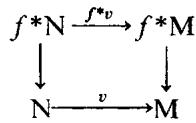
\includegraphics[keepaspectratio]{images/part001_e53c46a7.jpg}}

交换。

7.2.5. 设 B' 是 B 的子流形，i 是从 B' 到 B 的典范嵌入。若 M 是以 B 为基底的向量丛，则 \(i^*M\) 称为 M 在 B' 上诱导的向量丛，记为 \(M|_{B'}\)。若 \(t = (\mathrm{U}, \varphi, \mathrm{F})\) 是 M 的一个向量丛图，则 \((\mathrm{U} \cap \mathrm{B}', \varphi | \pi^{-1}(\mathrm{U} \cap \mathrm{B}'), \mathrm{F})\) 是 \(M|_{B'}\) 的一个向量丛图。从 \(M|_{B'}\) 到 M 的典范 f-态射是从 \(M|_{B'}\) 到 M 的子流形 \(\pi^{-1}(\mathrm{B}')\) 的一个流形同构。

7.2.6. 设 \(f\) 是从流形 B' 到 B 的态射，M（分别 M'）是以 B（分别 B'）为基底的向量丛。从 M 到 M' 的 \(f\)-余态射定义为从 \(f^{*}M\) 到 M' 的 B'-态射。当 B = B' 且 \(f = \mathrm{Id}_{\mathbf{B}}\) 时，从 M 到 M' 的 f-余态射的数据等价于从 M 到 M' 的 B-态射的数据。

设 \(g\) 是一个 \(f\)-余态射，从 \(\mathbf{M}\) 到 \(\mathbf{M}'\)。对每个 \(b \in \mathbf{B}'\)，映射 \(g_b: x \mapsto g(b, x)\) 从 \(\mathbf{M}_{f(b)}\) 到 \(\mathbf{M}_b'\)，是连续线性映射。

此外，设 \(f'\) 是从流形 \(B''\) 到 \(B'\) 的态射，且 \(h\) 是一个 \(f'\)-余态射，从 \(M'\) 到向量丛 \(M''\)，其基底为 \(B''\)。于是，映射 \(h \circ f'^{*}g\)，其定义域为 \(f'^{*}(f^{*}M) = (f \circ f')^{*}M\)，值域为 \(M''\)，是 \((f \circ f')\)-余态射，从 \(M\) 到 \(M''\)，记为 \(h \circ g\)。对于 \(b \in B''\)，有

\[
(h \circ g) _ {b} = h _ {b} \circ g _ {f ^ {\prime} (b)}.
\]

